\documentclass[]{book}
\usepackage{lmodern}
\usepackage{amssymb,amsmath}
\usepackage{ifxetex,ifluatex}
\usepackage{fixltx2e} % provides \textsubscript
\ifnum 0\ifxetex 1\fi\ifluatex 1\fi=0 % if pdftex
  \usepackage[T1]{fontenc}
  \usepackage[utf8]{inputenc}
\else % if luatex or xelatex
  \ifxetex
    \usepackage{mathspec}
  \else
    \usepackage{fontspec}
  \fi
  \defaultfontfeatures{Ligatures=TeX,Scale=MatchLowercase}
\fi
% use upquote if available, for straight quotes in verbatim environments
\IfFileExists{upquote.sty}{\usepackage{upquote}}{}
% use microtype if available
\IfFileExists{microtype.sty}{%
\usepackage{microtype}
\UseMicrotypeSet[protrusion]{basicmath} % disable protrusion for tt fonts
}{}
\usepackage[margin=1in]{geometry}
\usepackage{hyperref}
\hypersetup{unicode=true,
            pdftitle={Finn 6211 - Final Project},
            pdfauthor={Davis Vaughan},
            pdfborder={0 0 0},
            breaklinks=true}
\urlstyle{same}  % don't use monospace font for urls
\usepackage{natbib}
\bibliographystyle{apalike}
\usepackage{color}
\usepackage{fancyvrb}
\newcommand{\VerbBar}{|}
\newcommand{\VERB}{\Verb[commandchars=\\\{\}]}
\DefineVerbatimEnvironment{Highlighting}{Verbatim}{commandchars=\\\{\}}
% Add ',fontsize=\small' for more characters per line
\usepackage{framed}
\definecolor{shadecolor}{RGB}{248,248,248}
\newenvironment{Shaded}{\begin{snugshade}}{\end{snugshade}}
\newcommand{\AlertTok}[1]{\textcolor[rgb]{0.94,0.16,0.16}{#1}}
\newcommand{\AnnotationTok}[1]{\textcolor[rgb]{0.56,0.35,0.01}{\textbf{\textit{#1}}}}
\newcommand{\AttributeTok}[1]{\textcolor[rgb]{0.77,0.63,0.00}{#1}}
\newcommand{\BaseNTok}[1]{\textcolor[rgb]{0.00,0.00,0.81}{#1}}
\newcommand{\BuiltInTok}[1]{#1}
\newcommand{\CharTok}[1]{\textcolor[rgb]{0.31,0.60,0.02}{#1}}
\newcommand{\CommentTok}[1]{\textcolor[rgb]{0.56,0.35,0.01}{\textit{#1}}}
\newcommand{\CommentVarTok}[1]{\textcolor[rgb]{0.56,0.35,0.01}{\textbf{\textit{#1}}}}
\newcommand{\ConstantTok}[1]{\textcolor[rgb]{0.00,0.00,0.00}{#1}}
\newcommand{\ControlFlowTok}[1]{\textcolor[rgb]{0.13,0.29,0.53}{\textbf{#1}}}
\newcommand{\DataTypeTok}[1]{\textcolor[rgb]{0.13,0.29,0.53}{#1}}
\newcommand{\DecValTok}[1]{\textcolor[rgb]{0.00,0.00,0.81}{#1}}
\newcommand{\DocumentationTok}[1]{\textcolor[rgb]{0.56,0.35,0.01}{\textbf{\textit{#1}}}}
\newcommand{\ErrorTok}[1]{\textcolor[rgb]{0.64,0.00,0.00}{\textbf{#1}}}
\newcommand{\ExtensionTok}[1]{#1}
\newcommand{\FloatTok}[1]{\textcolor[rgb]{0.00,0.00,0.81}{#1}}
\newcommand{\FunctionTok}[1]{\textcolor[rgb]{0.00,0.00,0.00}{#1}}
\newcommand{\ImportTok}[1]{#1}
\newcommand{\InformationTok}[1]{\textcolor[rgb]{0.56,0.35,0.01}{\textbf{\textit{#1}}}}
\newcommand{\KeywordTok}[1]{\textcolor[rgb]{0.13,0.29,0.53}{\textbf{#1}}}
\newcommand{\NormalTok}[1]{#1}
\newcommand{\OperatorTok}[1]{\textcolor[rgb]{0.81,0.36,0.00}{\textbf{#1}}}
\newcommand{\OtherTok}[1]{\textcolor[rgb]{0.56,0.35,0.01}{#1}}
\newcommand{\PreprocessorTok}[1]{\textcolor[rgb]{0.56,0.35,0.01}{\textit{#1}}}
\newcommand{\RegionMarkerTok}[1]{#1}
\newcommand{\SpecialCharTok}[1]{\textcolor[rgb]{0.00,0.00,0.00}{#1}}
\newcommand{\SpecialStringTok}[1]{\textcolor[rgb]{0.31,0.60,0.02}{#1}}
\newcommand{\StringTok}[1]{\textcolor[rgb]{0.31,0.60,0.02}{#1}}
\newcommand{\VariableTok}[1]{\textcolor[rgb]{0.00,0.00,0.00}{#1}}
\newcommand{\VerbatimStringTok}[1]{\textcolor[rgb]{0.31,0.60,0.02}{#1}}
\newcommand{\WarningTok}[1]{\textcolor[rgb]{0.56,0.35,0.01}{\textbf{\textit{#1}}}}
\usepackage{longtable,booktabs}
\usepackage{graphicx,grffile}
\makeatletter
\def\maxwidth{\ifdim\Gin@nat@width>\linewidth\linewidth\else\Gin@nat@width\fi}
\def\maxheight{\ifdim\Gin@nat@height>\textheight\textheight\else\Gin@nat@height\fi}
\makeatother
% Scale images if necessary, so that they will not overflow the page
% margins by default, and it is still possible to overwrite the defaults
% using explicit options in \includegraphics[width, height, ...]{}
\setkeys{Gin}{width=\maxwidth,height=\maxheight,keepaspectratio}
\IfFileExists{parskip.sty}{%
\usepackage{parskip}
}{% else
\setlength{\parindent}{0pt}
\setlength{\parskip}{6pt plus 2pt minus 1pt}
}
\setlength{\emergencystretch}{3em}  % prevent overfull lines
\providecommand{\tightlist}{%
  \setlength{\itemsep}{0pt}\setlength{\parskip}{0pt}}
\setcounter{secnumdepth}{5}
% Redefines (sub)paragraphs to behave more like sections
\ifx\paragraph\undefined\else
\let\oldparagraph\paragraph
\renewcommand{\paragraph}[1]{\oldparagraph{#1}\mbox{}}
\fi
\ifx\subparagraph\undefined\else
\let\oldsubparagraph\subparagraph
\renewcommand{\subparagraph}[1]{\oldsubparagraph{#1}\mbox{}}
\fi

%%% Use protect on footnotes to avoid problems with footnotes in titles
\let\rmarkdownfootnote\footnote%
\def\footnote{\protect\rmarkdownfootnote}

%%% Change title format to be more compact
\usepackage{titling}

% Create subtitle command for use in maketitle
\newcommand{\subtitle}[1]{
  \posttitle{
    \begin{center}\large#1\end{center}
    }
}

\setlength{\droptitle}{-2em}
  \title{Finn 6211 - Final Project}
  \pretitle{\vspace{\droptitle}\centering\huge}
  \posttitle{\par}
  \author{Davis Vaughan}
  \preauthor{\centering\large\emph}
  \postauthor{\par}
  \predate{\centering\large\emph}
  \postdate{\par}
  \date{2018-04-12}

\usepackage{booktabs}

\begin{document}
\maketitle

{
\setcounter{tocdepth}{1}
\tableofcontents
}
\hypertarget{titlepage}{%
\chapter{Introduction}\label{titlepage}}

This is the final project of the Finn 6211 class, with the intention of
getting comfortable with spot rate data, their relation to yield curve
factors, and various hedging strategies.

The instructions for the report can be found
\href{./instructions/Hedging_Project_S18.pdf}{here}.

An R package has been created to accompany the report. It contains a
number of helper functions for cleaning data, manipulating the time
series, and creating the hedging strategies. The package is named,
\texttt{ratekit} and can be found on Github \href{}{here}.

This report was written with
\href{https://bookdown.org/yihui/bookdown/}{bookdown}, a book authoring
package for R.

\hypertarget{data}{%
\chapter{Data}\label{data}}

\hypertarget{retrieve}{%
\section{Getting the data}\label{retrieve}}

Script) \href{./R/01-download.R}{01-download.R}

The data is retrieved from the Federal Reserve website, under the
discussion series: \emph{The U.S. Treasury Yield Curve: 1961 to the
Present}. The link for that site is
\href{https://www.federalreserve.gov/pubs/feds/2006/200628/200628abs.html}{here}.
The specific data set that was downloaded was the XLS file included on
that site.

The data was immediately opened in Excel, and was resaved as an
\texttt{xlsx} file. The format of the data is not a true \texttt{xls}
file, instead it is some kind of \texttt{xml} file. This does not play
nicely with R's packages for importing Excel data, so a resave was
necessary and is done manually.

\texttt{ratekit} provides the \texttt{download\_rates\_xls()} helper
function for this.

\hypertarget{cleaning}{%
\section{Cleaning}\label{cleaning}}

Script) \href{./R/02-cleaning.R}{02-cleaning.R}

Data is brought in using the \texttt{readxl} package and the
\texttt{ratekit} helper, \texttt{read\_rates()}. This function reads the
rectangle of rates data only, and sets any \texttt{-999.99} values to
\texttt{NA}. These are often found through the dataset, and I assume
they are meant to represent missing values. To visualize the \texttt{NA}
values in the dataset, I use the \texttt{visdat} package.

First, let's look at what is immediately brought in by
\texttt{read\_rates()}. We will need a few packages throughout the
chapter, so let's load those now as well.

\begin{Shaded}
\begin{Highlighting}[]
\KeywordTok{library}\NormalTok{(visdat)}
\KeywordTok{library}\NormalTok{(ratekit)}
\KeywordTok{library}\NormalTok{(dplyr)}
\KeywordTok{library}\NormalTok{(tibbletime)}

\NormalTok{raw <-}\StringTok{ }\KeywordTok{read_rates}\NormalTok{(}\StringTok{"data/raw/feds200628.xlsx"}\NormalTok{)}

\NormalTok{raw}
\end{Highlighting}
\end{Shaded}

\begin{verbatim}
## # A tibble: 14,163 x 100
##    date       SVENY01 SVENY02 SVENY03 SVENY04 SVENY05 SVENY06 SVENY07
##    <date>       <dbl>   <dbl>   <dbl>   <dbl>   <dbl>   <dbl>   <dbl>
##  1 2018-03-29    2.10    2.27    2.40    2.49    2.56    2.62    2.66
##  2 2018-03-28    2.10    2.28    2.41    2.51    2.59    2.65    2.69
##  3 2018-03-27    2.09    2.26    2.40    2.50    2.58    2.64    2.69
##  4 2018-03-26    2.10    2.30    2.45    2.57    2.65    2.71    2.76
##  5 2018-03-23    2.09    2.27    2.42    2.53    2.61    2.68    2.73
##  6 2018-03-22    2.09    2.29    2.44    2.55    2.63    2.70    2.74
##  7 2018-03-21    2.11    2.32    2.47    2.59    2.68    2.75    2.81
##  8 2018-03-20    2.12    2.34    2.49    2.61    2.69    2.75    2.80
##  9 2018-03-19    2.11    2.31    2.45    2.57    2.65    2.72    2.77
## 10 2018-03-16    2.10    2.30    2.45    2.56    2.65    2.71    2.76
## # ... with 14,153 more rows, and 92 more variables: SVENY08 <dbl>,
## #   SVENY09 <dbl>, SVENY10 <dbl>, SVENY11 <dbl>, SVENY12 <dbl>,
## #   SVENY13 <dbl>, SVENY14 <dbl>, SVENY15 <dbl>, SVENY16 <dbl>,
## #   SVENY17 <dbl>, SVENY18 <dbl>, SVENY19 <dbl>, SVENY20 <dbl>,
## #   SVENY21 <dbl>, SVENY22 <dbl>, SVENY23 <dbl>, SVENY24 <dbl>,
## #   SVENY25 <dbl>, SVENY26 <dbl>, SVENY27 <dbl>, SVENY28 <dbl>,
## #   SVENY29 <dbl>, SVENY30 <dbl>, SVENPY01 <dbl>, SVENPY02 <dbl>,
## #   SVENPY03 <dbl>, SVENPY04 <dbl>, SVENPY05 <dbl>, SVENPY06 <dbl>,
## #   SVENPY07 <dbl>, SVENPY08 <dbl>, SVENPY09 <dbl>, SVENPY10 <dbl>,
## #   SVENPY11 <dbl>, SVENPY12 <dbl>, SVENPY13 <dbl>, SVENPY14 <dbl>,
## #   SVENPY15 <dbl>, SVENPY16 <dbl>, SVENPY17 <dbl>, SVENPY18 <dbl>,
## #   SVENPY19 <dbl>, SVENPY20 <dbl>, SVENPY21 <dbl>, SVENPY22 <dbl>,
## #   SVENPY23 <dbl>, SVENPY24 <dbl>, SVENPY25 <dbl>, SVENPY26 <dbl>,
## #   SVENPY27 <dbl>, SVENPY28 <dbl>, SVENPY29 <dbl>, SVENPY30 <dbl>,
## #   SVENF01 <dbl>, SVENF02 <dbl>, SVENF03 <dbl>, SVENF04 <dbl>,
## #   SVENF05 <dbl>, SVENF06 <dbl>, SVENF07 <dbl>, SVENF08 <dbl>,
## #   SVENF09 <dbl>, SVENF10 <dbl>, SVENF11 <dbl>, SVENF12 <dbl>,
## #   SVENF13 <dbl>, SVENF14 <dbl>, SVENF15 <dbl>, SVENF16 <dbl>,
## #   SVENF17 <dbl>, SVENF18 <dbl>, SVENF19 <dbl>, SVENF20 <dbl>,
## #   SVENF21 <dbl>, SVENF22 <dbl>, SVENF23 <dbl>, SVENF24 <dbl>,
## #   SVENF25 <dbl>, SVENF26 <dbl>, SVENF27 <dbl>, SVENF28 <dbl>,
## #   SVENF29 <dbl>, SVENF30 <dbl>, SVEN1F01 <dbl>, SVEN1F04 <dbl>,
## #   SVEN1F09 <dbl>, BETA0 <dbl>, BETA1 <dbl>, BETA2 <dbl>, BETA3 <dbl>,
## #   TAU1 <dbl>, TAU2 <dbl>
\end{verbatim}

Not a bad start, but I'm worried about missing values. Also, what are
those column names?

The column names in the data correspond to different types and lengths
of rates used in the paper. The key for understanding the column names
is below:

\begin{tabular}{l|l|l}
\hline
series & compounding\_convention & key\\
\hline
Zero-coupon yield & Continuously Compounded & SVENYXX\\
\hline
Par yield & Coupon-Equivalent & SVENPYXX\\
\hline
Instantaneous forward rate & Continuously Compounded & SVENFXX\\
\hline
One-year forward rate & Coupon-Equivalent & SVEN1FXX\\
\hline
Parameters & NA & BETA0 to TAU2\\
\hline
\end{tabular}

Using \texttt{vis\_dat()}, we can take a look at our dataset all at once
to determine which data points to exclude.

\begin{Shaded}
\begin{Highlighting}[]
\KeywordTok{vis_dat}\NormalTok{(raw, }\DataTypeTok{warn_large_data =} \OtherTok{FALSE}\NormalTok{)}
\end{Highlighting}
\end{Shaded}

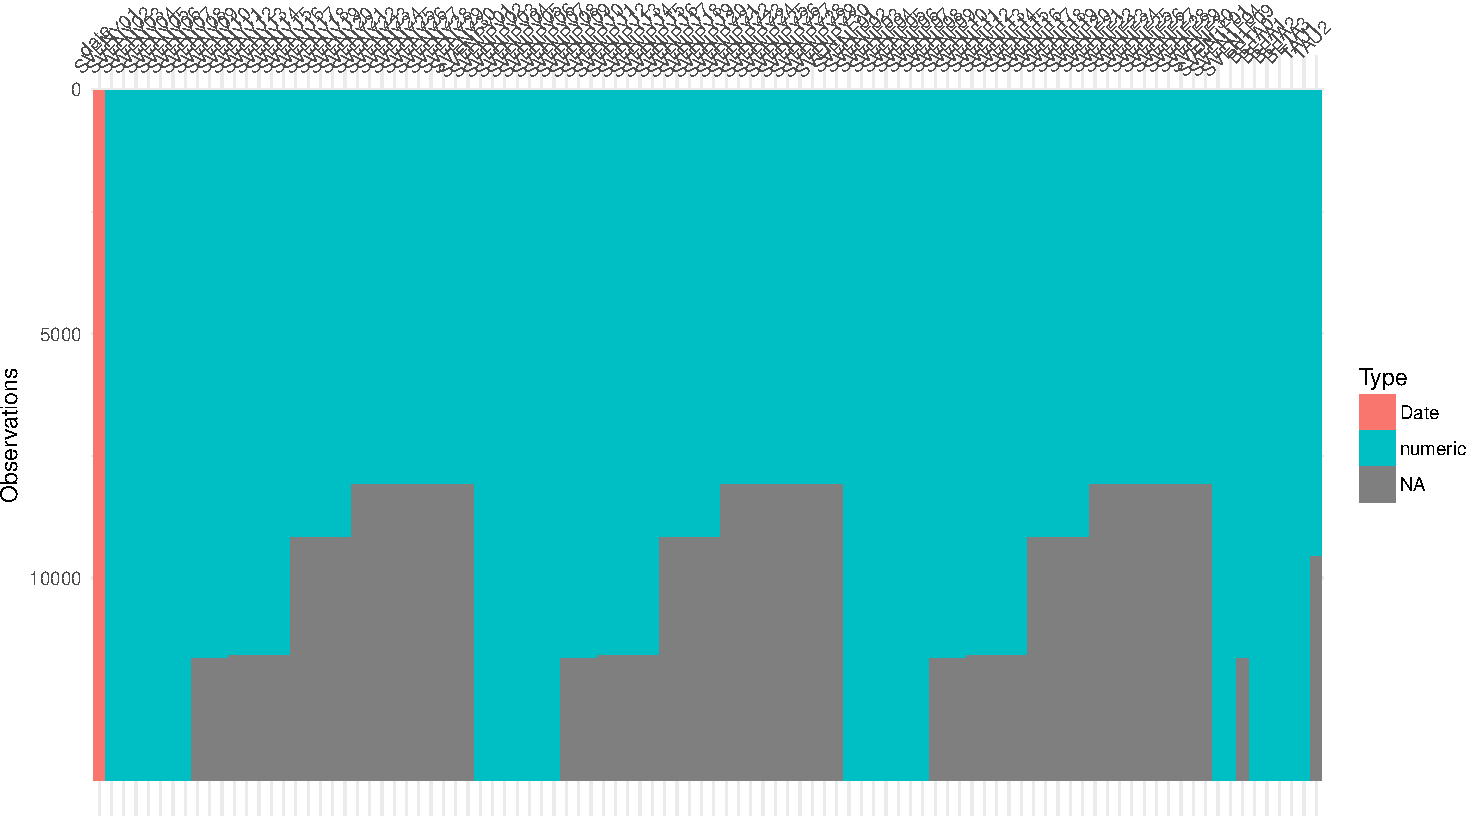
\includegraphics{final-project-book_files/figure-latex/missing_vals-1.pdf}

A clear pattern is seen in the missing values, with the number of
missing values increasing as you go further back in time and look at
longer rates (10 year VS 30 year). This might be a bit difficult to see
if you look at everything, but becomes clearer if you zoom in on just
one set of series.

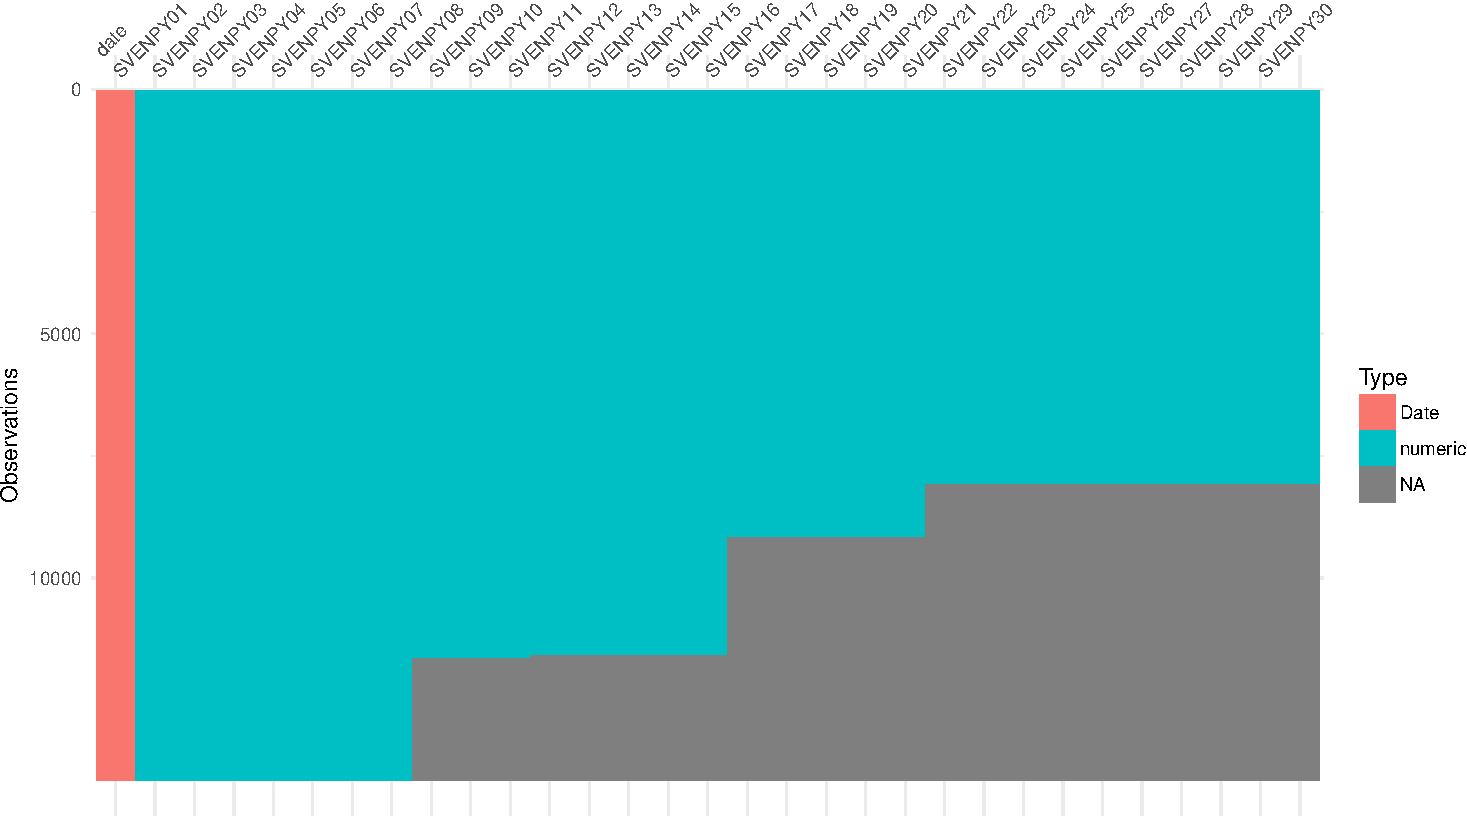
\includegraphics{final-project-book_files/figure-latex/par_yield_missing-1.pdf}

The parameters are affected by this as well, but not as much, with only
\texttt{TAU2} being affected.

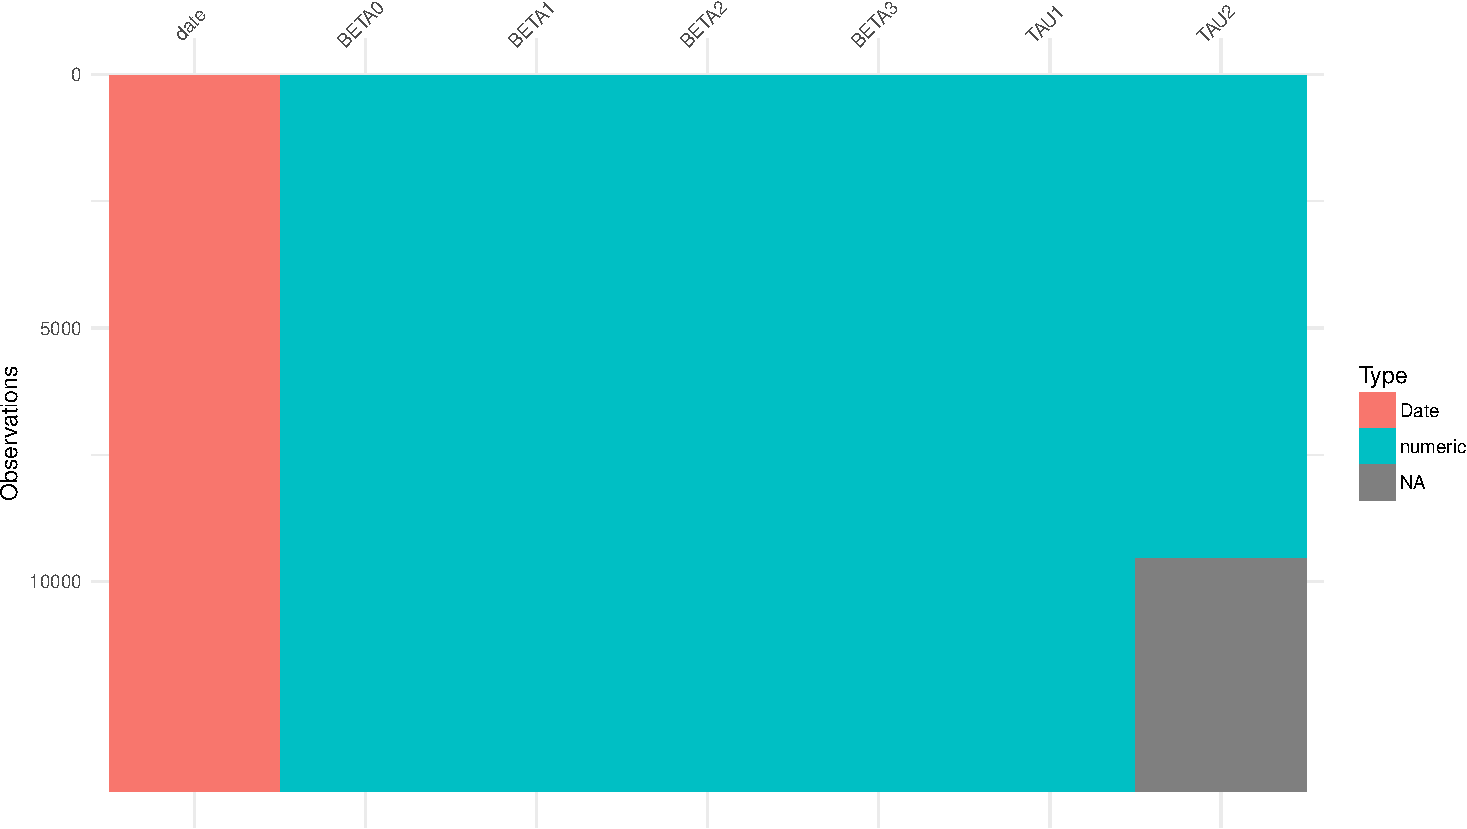
\includegraphics{final-project-book_files/figure-latex/parameters_missing-1.pdf}

Since the parameters are all we care about for this project, I decided
to throw out any row with an \texttt{NA} value for \texttt{TAU2}. This
threw out every data point before 1980. We can ensure that we don't have
any missing values now with \texttt{vis\_miss()}.

\begin{Shaded}
\begin{Highlighting}[]
\CommentTok{# This is the cleaned parameter set, cleaned using 02-cleaning.R}
\NormalTok{parameters <-}\StringTok{ }\KeywordTok{readRDS}\NormalTok{(}\StringTok{"data/cleaned/parameters/parameters.rds"}\NormalTok{)}
\KeywordTok{vis_miss}\NormalTok{(parameters)}
\end{Highlighting}
\end{Shaded}

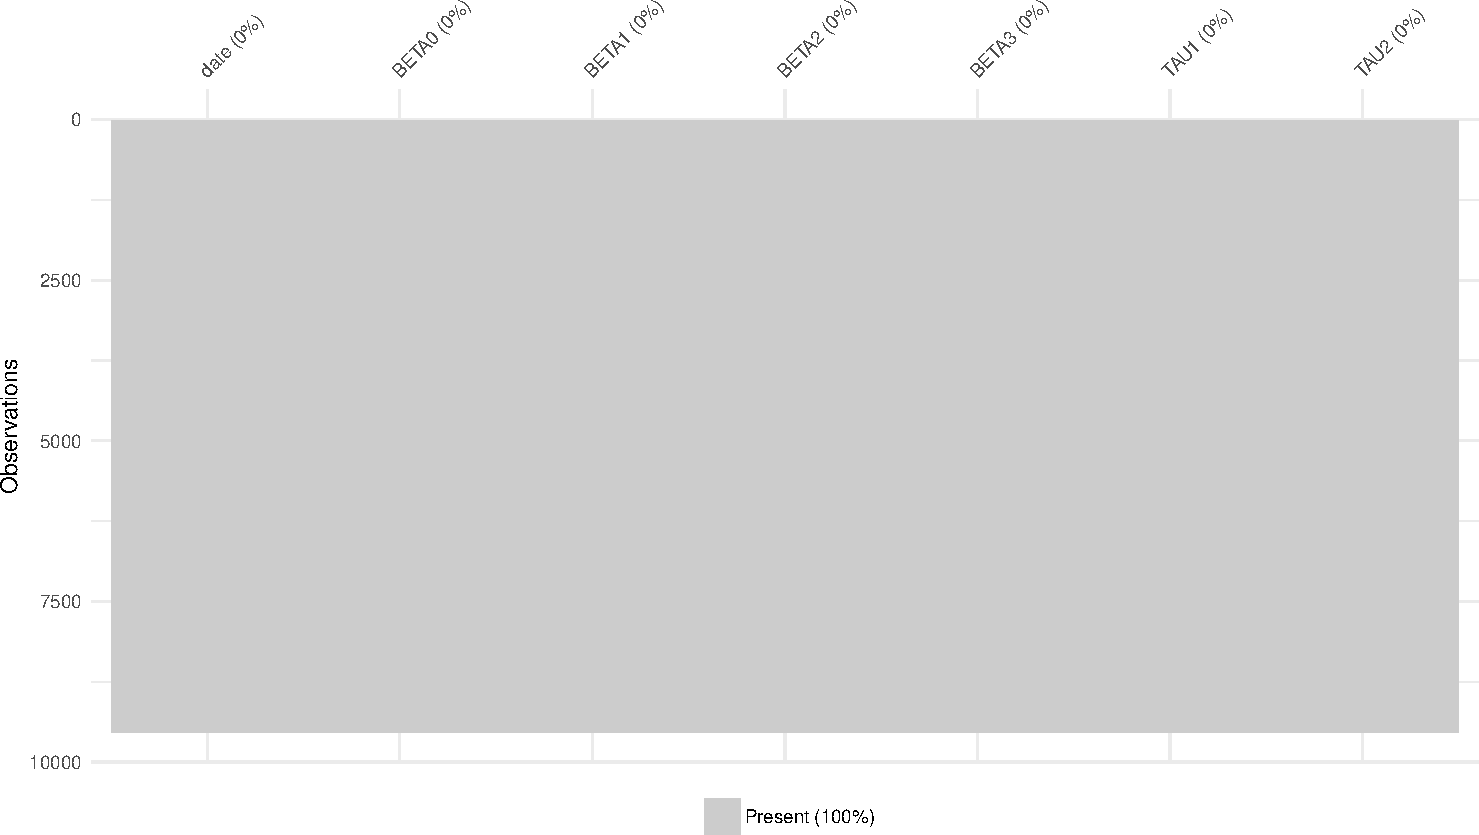
\includegraphics{final-project-book_files/figure-latex/parameters_clean-1.pdf}

\hypertarget{monthly}{%
\section{Monthly and Ascending}\label{monthly}}

Script)
\href{./R/03-to-monthly-and-ascending.R}{03-to-monthly-and-ascending.R}

At this point, our dataset looks like this:

\begin{Shaded}
\begin{Highlighting}[]
\NormalTok{parameters <-}\StringTok{ }\KeywordTok{readRDS}\NormalTok{(}\StringTok{"data/cleaned/parameters/parameters.rds"}\NormalTok{)}
\NormalTok{parameters}
\end{Highlighting}
\end{Shaded}

\begin{verbatim}
## # A tibble: 9,543 x 7
##    date       BETA0 BETA1      BETA2 BETA3  TAU1  TAU2
##    <date>     <dbl> <dbl>      <dbl> <dbl> <dbl> <dbl>
##  1 2018-03-29  4.13 -2.25  0.000228  -3.07  2.84  11.4
##  2 2018-03-28  4.35 -2.48 -0.0000890 -3.53  2.99  12.2
##  3 2018-03-27  4.44 -2.59  0.000314  -3.67  3.18  12.5
##  4 2018-03-26  4.27 -2.44 -0.0000588 -3.12  2.73  11.8
##  5 2018-03-23  4.53 -2.69  0.000245  -3.78  3.17  12.9
##  6 2018-03-22  4.31 -2.48 -0.000162  -3.31  2.78  11.9
##  7 2018-03-21  4.80 -2.95 -0.550     -4.41  2.55  13.1
##  8 2018-03-20  4.04 -2.21 -0.0000964 -2.43  2.43  10.8
##  9 2018-03-19  4.66 -2.80  0.00297   -4.10  3.12  13.0
## 10 2018-03-16  4.61 -2.78  0.000246  -4.02  3.03  12.9
## # ... with 9,533 more rows
\end{verbatim}

We want monthly data, and we will need to put it in ascending order. We
can convert to monthly with \texttt{as\_period()} from
\texttt{tibbletime}, and arrange it by ascending date with
\texttt{arrange()} from \texttt{dplyr}.

\begin{Shaded}
\begin{Highlighting}[]
\NormalTok{parameters_monthly <-}\StringTok{ }\NormalTok{parameters }\OperatorTok
\StringTok{  }\KeywordTok{as_tbl_time}\NormalTok{(date) }\OperatorTok
\StringTok{  }\KeywordTok{arrange}\NormalTok{(date) }\OperatorTok\StringTok{ }
\StringTok{  }\KeywordTok{as_period}\NormalTok{(}\StringTok{"monthly"}\NormalTok{, }\DataTypeTok{side =} \StringTok{"end"}\NormalTok{)}

\NormalTok{parameters_monthly}
\end{Highlighting}
\end{Shaded}

\begin{verbatim}
## # A time tibble: 459 x 7
## # Index: date
##    date       BETA0   BETA1 BETA2 BETA3  TAU1  TAU2
##    <date>     <dbl>   <dbl> <dbl> <dbl> <dbl> <dbl>
##  1 1980-01-31  11.8   0.979 -622.  617. 2.50  2.50 
##  2 1980-02-29  11.8   1.53  -617.  621. 1.15  1.15 
##  3 1980-03-31  13.2   2.95  -622.  617. 1.78  1.76 
##  4 1980-04-30  11.1   0.607 -621.  617. 1.59  1.59 
##  5 1980-05-30  11.3  -3.44  -620.  618. 1.36  1.35 
##  6 1980-06-30  25.0 -17.0   -631.  607. 6.20  6.06 
##  7 1980-07-31  16.6  -8.33  -624.  615. 3.81  3.76 
##  8 1980-08-29  19.6  -8.94  -627.  612. 5.04  4.94 
##  9 1980-09-30  13.0  -1.34  -621.  618. 2.21  2.20 
## 10 1980-10-31  11.9   1.06  -618.  620. 0.379 0.379
## # ... with 449 more rows
\end{verbatim}

This leaves us with 459 rows of data for our project, spanning
1980-01-31 to 2018-03-29.

\hypertarget{rates}{%
\chapter{Fixed Income Features Calculations}\label{rates}}

\bibliography{book.bib,packages.bib}


\end{document}
